% !TEX root = regularized.tex
The described methods have been implemented and tested using MATLAB R2020a and the toolboxes AIR Tools II \cite{art:HANS18} and IR Tools \cite{art:GAZZ19}. We stop the outer iteration when
\[
\|L x^{(\ell)}\|_2^2 < \|L x^{(\ell-1)}\|_2^2,
\]
as proposed in \cite{Gazzola_etal_2020}. The multigrid preconditioned GMRES was used without restarting and with an absolute residual stopping criterion of $10^{-6}$.

\subsection{Effect of pre- and post-smoothing}
Before evaluating the proposed method in detail, we study the dependence of the convergence rate on the number of pre- and post-smoothing steps. For that purpose, we study a tomography example using the Shepp Logan phantom of size $128 \times 128$ with 1\% added noise, created using IR Tools' \cite{art:GAZZ19} \texttt{PRtomo} and \texttt{PRnoise} routines. We tested V(0,1)-, V(1,1)-, V(1,2)-, V(2,1)- and V(2,2)-cycles for this problem. For each outer iteration we recorded the minimal, maximal and average number of inner iterations needed for the different values of $\lambda$ that where evaluated in the respective outer iteration. The resulting maximal, minimal and average numbers of iterations is depicted in Fig.~\ref{fig:its_cycling}, the average number of iterations needed in each outer iteration can also be found in Table~\ref{tab:its_cycling}. As can be seen the difference between V(2,1) cycles and V(2,2) cycles is small and the former even perform better for early outer iterations. Therefore we decided to use V(2,1) cycles in the rest our numerical experiments.
\begin{figure}[htbp]
\begin{center}
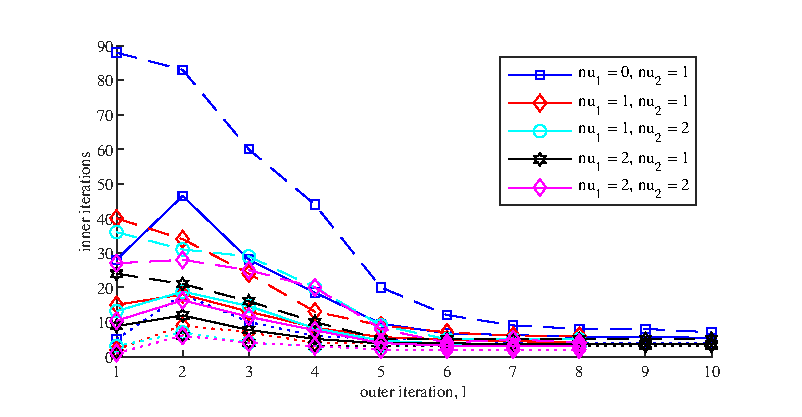
\includegraphics{figures/its_cycling}
\caption{Number of inner iterations needed in each outer iterations of the method applied to the Shepp Logan phantom of size $128 \times 128$ with 1\% noise for different multigrid cycles. Solid lines represent the average number of iterations needed for the different values of lambda, dashed lines the maximum and dotted lines the minimum.}
\label{fig:its_cycling}
\end{center}
\end{figure}
\begin{table}[htp]
\caption{Average number of inner iterations needed in each outer iterations of the method applied to the Shepp Logan phantom of size $128 \times 128$ with 1\% noise for different multigrid cycles.}
\begin{center}
\begin{tabular}{|l|r|r|r|r|r|r|r|r|r|r|}
\hline
& \multicolumn{1}{c|}{1} & \multicolumn{1}{c|}{2} & \multicolumn{1}{c|}{3} & \multicolumn{1}{c|}{4} & \multicolumn{1}{c|}{5} & \multicolumn{1}{c|}{6} & \multicolumn{1}{c|}{7} & \multicolumn{1}{c|}{8} & \multicolumn{1}{c|}{9} & \multicolumn{1}{c|}{10} \\
\hline
V(0,1) & 28.0 & 46.5 & 28.1 & 18.5 & 9.5 & 6.7 & 6.2 & 5.7 & 5.7 & 5.4 \\
V(1,1) & 15.0 & 18.0 & 13.0 & 8.4 & 5.6 & 5.0 & 4.4 & 4.2 & \multicolumn{1}{c|}{---} & \multicolumn{1}{c|}{---}\\
V(1,2) & 13.1 & 18.8 & 14.6 & 8.2 & 4.6 & 3.7 & 3.5 & 3.4 & \multicolumn{1}{c|}{---} & \multicolumn{1}{c|}{---} \\
V(2,1) & 8.8 & 11.9 & 7.7 & 5.1 & 3.8 & 3.8 & 3.7 & 3.7 & 3.6 & 3.6 \\
V(2,2) & 10.4 &16.3 & 11.5 & 7.6 & 3.9 & 3.1 & 3.0 & 2.9 & \multicolumn{1}{c|}{---} & \multicolumn{1}{c|}{---} \\
\hline
\end{tabular}
\end{center}
\label{tab:its_cycling}
\end{table}%


%As a first example we consider the Shepp-Logan phantom, generated by
%the MATLAB command \texttt{phantom}. We consider a version of size
%$64^2$ with added noise of level $0.5\%$, $1\%$ and $2\%$. The
%iteration was stopped, when the regularization error of the current
%solution $x^{(k)}$, measured as the 2-norm of $L^TW^2L$ applied to it,
%grew again, i.e., when
%\[
%  \| L^TW^2L x^{(k)} \|_2 > \| L^TW^2L x^{(k-1)} \|_2.
%\]
%In this case, the previous solution $x^{(k-1)}$ usually provides a
%good reconstruction.
%
%First, we ran the proposed algorithm for a full-angle Radon transform
%with 30 fixed values of $\lambda$, logarithmically spaced between
%$10^{-3}$ and $10^2$. The $\lambda$ chosen in each iteration can be
%found in Table~\ref{tab:chosen_lambda_all_lambda_full_angle}.
%
%\begin{table}
%  \begin{center}
%    \begin{tabular}{c|ccc|ccc}
%      Problem & \multicolumn{3}{|c}{full angle case} &
%                                                       \multicolumn{3}{|c}{limited
%                                                       angle case} \\
%      Noise & $0.5\%$ & $1\%$ & $2\%$ & $0.5\%$ & $1\%$ & $2\%$ \\
%      \hline
%      Iteration 1 & 0.0161 & 0.0356 & 0.0530 & 0.0161 & 0.0356 & 0.0530 \\
%      Iteration 2 & 0.0240 & 0.0530 & 0.0788 & 0.0240 & 0.0356 & 0.0788 \\
%      Iteration 3 & 0.0530 & 0.1172 & 0.2593 & 0.0356 & 0.0788 & 0.1172 \\
%      Iteration 4 & 0.0788 & 0.1743 & 0.3857 & 0.0530 & 0.1172 & 0.1743 \\
%      Iteration 5 & 0.1743 & 0.3857 & 0.8532 & 0.0788 & 0.1172 & 0.5736 \\
%      Iteration 6 & 0.3857 & 1.2690 & 1.2690 & 0.0788 & 0.1743 & 0.8532 \\
%      Iteration 7 & 1.2690 & 1.8874 & 2.8072 & 0.1172 & 0.2593 & 1.2690 \\
%      Iteration 8 & 2.8072 & 2.8072 & 6.2102 & 0.1172 & 0.5736 & 1.8874 \\
%      Iteration 9 & 6.2102 & 6.2102 & 9.2367 & 0.1743 & 0.8532 & 2.8072 \\
%      Iteration 10 & 13.7382 & 13.7382 & 13.7382 & 0.2593 & 1.2690 & 6.2102 \\
%      Iteration 11 & 30.3920 & 20.4336 & 30.3920 & 0.3857 & 1.8874 & 6.2102 \\
%      Iteration 12 & 67.2336 & 45.2035 & 67.2336 & 0.5736 & 1.8874 & 13.7382 \\
%      Iteration 13 & 67.2336 & 67.2336 & 67.2336 & 1.2690 & 2.8072 & 20.4336 \\
%      Iteration 14 & 2.8072 & 67.2336 & 67.2336 & 2.8072 & 4.1753 & 30.3920 \\
%      Iteration 15 & --- & 67.2336 & 67.2336 & 6.2102 & 6.2102 & 45.2035 \\
%      Iteration 16 & --- & 67.2336 & 6.2102 & 13.7382 & 13.7382 & 67.2336 \\
%      Iteration 17 & --- & 6.2102 & --- & 30.3920 & 30.3902 & 67.2336 \\
%      Iteration 18 & --- & --- & --- & 67.2336 & 67.2336 & 67.2336 \\
%      Iteration 19 & --- & --- & --- & 67.2336 & 67.2336 & 67.2336 \\
%      Iteration 20 & --- & --- & --- & 67.2336 & 67.2336 & 67.2336 \\
%      Iteration 21 & --- & --- & --- & 4.1753 & 4.1753 & 67.2336 \\
%      Iteration 22 & --- & --- & --- & --- & --- & 13.7382 \\
%    \end{tabular}
%  \end{center}
%  \caption{Chosen $\lambda$ in each iteration for different noise
%    levels for the full angle case.}
%  \label{tab:chosen_lambda_all_lambda_full_angle}
%\end{table}

% \subsection{Deblurring?}

% \subsection{Radon Transform}

% Current example.  Play with noise level (once L-curve selection is
% back in).

% \subsection{Another example?}

